%%%%%%%%%%%%%%%%%%%%%%%%%%%%%%%%%%%%%%%%%%%%%%%%%%%%%%%%%%%%%%%%%%%%%%%%%%%%%%%
%%%%%%%%%%%%%%%%%%%%%%%%%%%%%%%%%%%%%%%%%%%%%%%%%%%%%%%%%%%%%%%%%%%%%%%%%%%%%%%
%%%%%%%%%%%%%%%%%%%%%%%%%%%%%%%%%%%%%%%%%%%%%%%%%%%%%%%%%%%%%%%%%%%%%%%%%%%%%%%
%% Marco Sgobino
%% Tesi di laurea triennale

\documentclass[a4paper, 12pt]{report}

\usepackage[T1]{fontenc}
\usepackage[utf8]{inputenc}
\usepackage[italian]{babel}
\usepackage{graphicx} % Manage pictures
\usepackage{hyperref} % Reference Links
\usepackage{times} % Times font

\usepackage{color} % Allows defining colors
\usepackage{setspace} % Sets leading
\usepackage[a4paper, inner=0.5cm, outer=0.5cm, lmargin=2cm, rmargin=2cm, tmargin=2.5cm, bmargin=2cm]{geometry} % Sets margins

% This will change "\chapter" style into 'N CHAPTER NAME'
\usepackage{titlesec}
\titleformat{\chapter}[display]
{\Huge\bfseries}{}{0pt}{\thechapter\ \ \ \ }


% Code customization
\usepackage{listings}
\definecolor{dkgreen}{rgb}{0.1,0.5,0.1}
\definecolor{greengray}{rgb}{0.32,0.57,0.32}
\definecolor{orange}{rgb}{0.96,0.42,0}
\definecolor{lightblue}{rgb}{0,0.28,0.95}
\definecolor{background}{rgb}{0.995,0.995,0.995}
\lstset {
        frame=tb,
        language=[5.2]Lua,
        aboveskip=3mm,
        belowskip=3mm,
        showstringspaces=false,
        columns=flexible,
        basicstyle={\small\ttfamily},
        numbers=none,
        backgroundcolor=\color{background},
        numberstyle=\tiny\color{drkgeen},
        keywordstyle=\color{lightblue},
        commentstyle=\color{greengray},
        stringstyle=\color{orange},
        breaklines=true,
        breakatwhitespace=true,
        tabsize=3
}

\setlength{\parindent}{28.35pt}

%%%%%%%%%%%%%%%%%%%%%%%%%%%%%%%%%%%%%%%%%%%%%%%%%%%%%%%%%%%%%%%%%%%%%%%%%%%%%%%
%%%%%%%%%%%%%%%%%%%%%%%%%%%%%%%%%%%%%%%%%%%%%%%%%%%%%%%%%%%%%%%%%%%%%%%%%%%%%%%
%%%%%%%%%%%%%%%%%%%%%%%%%%%%%%%%%%%%%%%%%%%%%%%%%%%%%%%%%%%%%%%%%%%%%%%%%%%%%%%

\begin{document}

\title{Script Lua per controllo remoto droni}
\author{Marco Sgobino}
\maketitle % Prints title
\tableofcontents % Prints table of contents
\fontsize{12pt}{14pt}\selectfont
\setstretch{1.5} % Sets leading to 1.5

%% Frontespizio
%% Indice
\chapter{PREMESSA}
L'obiettivo di questa tesi sperimentale è stato quello di realizzare degli script in Lua per OpenTX, un firmware per radiocomandi open source, specificatamente per i modelli di radiocomando \emph{RadioMaster TX16S} e \emph{Taranis QX7S}.


\chapter{INTRODUZIONE}
\chapter{MATERIALI E METODI}
% In questa sezione saranno presentati i materiali ed i metodi adottati durante la sperimentazione.
        \section{OpenTX}

        OpenTX \cite{opentx-github} è un firmware open source per radiocomandi, scritto in C++, con supporto per oltre 20 modelli di trasmittenti radio \cite{opentx-radios}.
        Lo sviluppo del software è gestito da una comunità di programmatori e piloti di aeromodelli e droni, ed il firmware è disponibile preinstallato in radiocomandi di vari produttori, fra cui \emph{FrSky} e \emph{RadioMaster}, aziende che hanno realizzato i due modelli adottati nella sperimentazione, il \emph{Taranis FrSky QX7S} ed il \emph{RadioMaster TX16S}.

        Il firmware si occupa sia di gestire l'input proveniente dagli slider (cursori), stick (leve), switch (interruttori) e knob (manopole) che compongono il telecomando producendo degli output nei 32 canali di trasmissione radio, sia di fornire un'interfaccia grafica su uno schermo LCD. Esso consente la configurazione completa della radio, dei modelli salvati in memoria su un supporto SD, o la visualizzazione di telemetria e dati ulteriori, come la batteria residua del radiocomando, la posizione mediante GPS, o l'indicatore \emph{RSSI} della potenza del segnale in ricezione. In aggiunta a ciò, è possibile riprodurre file audio dall'altoparlante della ricetrasmittente per creare annunci personalizzati ed aiutare il pilota con feedback vocali durante le sessioni di volo.


\begin{figure}[ht]
        \centering
        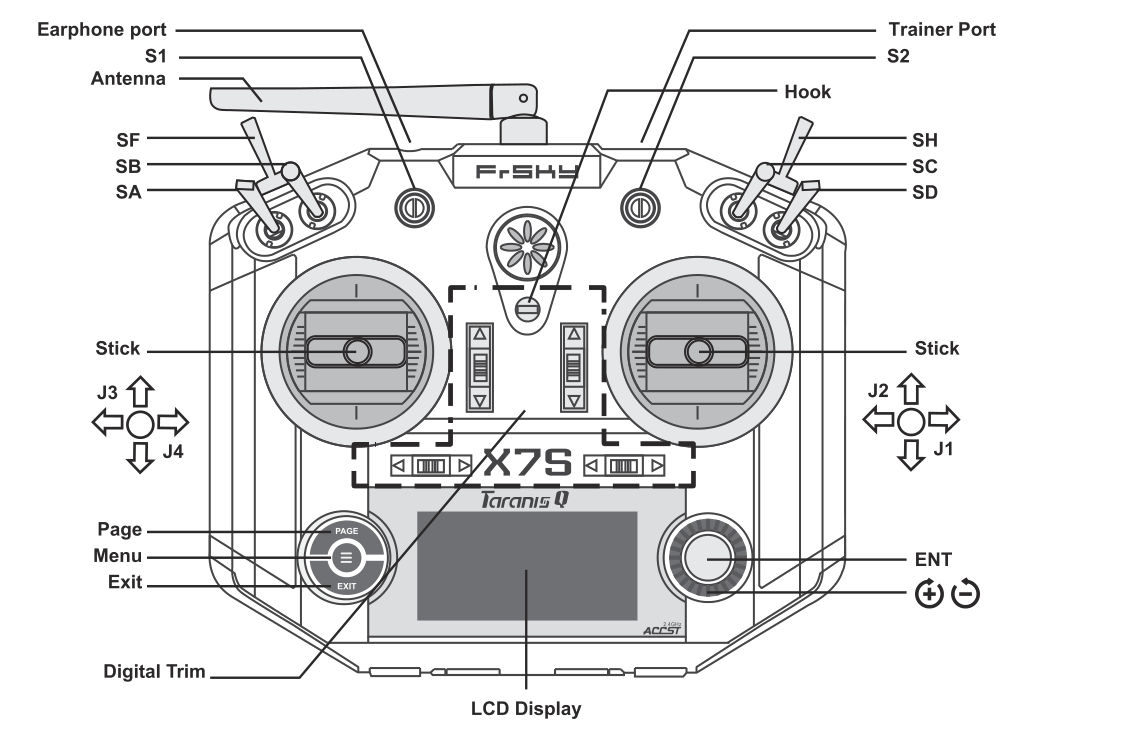
\includegraphics[ width=0.80\linewidth, height=\textheight, keepaspectratio]{./Pictures/qx7s-sticks.png}
        \caption{\footnotesize Leve e cursori dal manuale del \emph{Taranis QX7S}.}
        \label{fig:qx7s-sticks}
\end{figure}

OpenTX rende inoltre disponibile un software ad interfaccia grafica, \emph{OpenTX Companion} \cite{opentx-website}, disponibile per Windows, Mac OS e Linux. Tale software velocizza e facilita la configurazione del radiocomando con l'ausilio di un computer e consente di svolgere varie operazioni, fra cui:
\begin{itemize}
        \item scaricare ed installare il firmware OpenTX per il proprio radiocomando;
        \item modificare le configurazioni del radiocomando e dei modelli;
        \item eseguire backup delle configurazioni e ripristinarle all'occorrenza;
        \item modificare la schermata d'avvio del radiocomando;
        \item simulare i radiocomandi ed i modelli tramite il software \emph{OpenTX Simulator}.
\end{itemize}

\subsection{Gestione degli input ed elaborazione degli output mediante i mixer}\label{subsec:inputs-mixers-outputs}

OpenTX gestisce gli input e l'output e la loro elaborazione tramite \emph{cicli di calcolo} eseguiti varie volte al secondo; con ogni ciclo vengono lette le posizioni dei controlli, elaborati i \emph{mixer} e trasmessi gli output nei corretti canali di trasmissione radio. Tutto ciò avviene con sufficiente rapidità da garantire una risposta più rapida possibile alle variazioni degli input e da simulare una continuità nel tempo di tale risposta.

\subsubsection{Le sorgenti}
Le \emph{sorgenti} sono l'insieme delle leve, manopole e cursori che compongono i controlli del radiocomando. L'input viene letto assegnando alla posizione di ciascuno di essi un valore numerico:
\begin{itemize}
        \item un valore continuo da $-100$ a $+100$ per gli stick, gli slider ed i knob. Gli stick sono indicati con \emph{Ele} (Elevator stick), \emph{Ail} (Aileron stick), \emph{Thr} (Throttle stick) e \emph{Rud} (Rudder stick). Quando uno stick è collocato nella sua posizione centrale, il suo valore di input è pari a $0$. I knob invece sono indicati con \emph{S1} ed \emph{S2} (in alcuni radiocomandi con \emph{F1} ed \emph{F2}) e si tratta di manopole la cui funzione può essere liberamente impostata dall'utente. Gli slider di destra e sinistra (LS, RS) sono invece i potenziometri per gli stick, rispettivamente, di destra e di sinistra;
        \item $-100$, $0$ oppure $100$ per gli switch. Sono indicati con \emph{SA, SB, SC} e così via. Sono azionabili su tre posizioni: interruttore al centro (valore $0$), interruttore giù (valore $100$) ed interruttore su (valore $-100$);

        \item $100$ oppure $0$ per gli slider con solo due posizioni (presenti soltanto in alcuni modelli).
\end{itemize}

\subsubsection{I Mixer}
L'input proveniente dalle sorgenti viene elaborato ed inviato ai canali di output attraverso i \emph{mixer}. Ciascun mixer rappresenta l'\emph{interazione fra uno o più input ed uno o più output}. I mixer sono in grado di attribuire un \emph{peso} ai valori d'ingresso applicando al valore del segnale un coefficiente espresso con una percentuale, e di assegnare al segnale risultante almeno un canale di output. È possibile creare configurazioni combinando l'azione di più mixer per l'elaborazione dei vari input.
Un esempio è quello di impostare gli input dei quattro stick verso 4 canali di output, facendo in modo che il movimento completo dello stick produca un movimento completo del servo nel modello. Una possibile configurazione per tale scenario fa uso di $4$ mixer, ed è la seguente:

\begin{lstlisting}
        Configurazione dei canali di output
        Canale          Input           Mixer
        CH1             I1:Rud          Weight (+100%)
        CH2             I2:Ele          Weight (+100%)
        CH3             I3:Thr          Weight (+100%)
        CH4             I4:Ail          Weight (+100%)
\end{lstlisting}

Per l'input \texttt{Rud} è stato assegnato l'output nel canale \texttt{CH1} con peso \texttt{+100\%}, per l'input \texttt{Ele} è stato assegnato l'output nel canale \texttt{CH2} anch'esso con peso \texttt{+100\%}, e così via per gli altri due input \texttt{Thr} ed \texttt{Ail}.

Opzioni alternative potrebbero essere quelle di ridurre l'effetto dei singoli stick, dando ad essi un peso minore (ad esempio la metà, $50\%$), oppure invertire il segno del peso di modo da produrre un movimento del servo nella direzione opposta.

È inoltre possibile impostare un \emph{offset} per il valore in uscita, mediante la formula
$$\mbox{output } = \mbox{ sorgente} \cdot \mbox{peso } + \mbox{ offset }.$$

In aggiunta ai \emph{pesi} e agli \emph{offset}, OpenTX consente di valutare le sorgenti attraverso varie funzioni più complesse:
\begin{itemize}
        \item \emph{Diff}: riduce l'effetto dello stick in una direzione;
        \item \emph{Expo}: applica una curva esponenziale al segnale di input;
        \item \emph{Function}: applica una funzione matematica, o una disuguaglianza al segnale. Le funzioni sono in grado, ad esempio, di fornire in uscita il valore assoluto del segnale d'ingresso, oppure di prelevare l'input soltanto nel caso esso sia positivo $(x>0)$.
        \item \emph{Curve}: applica una curva impostata dall'utente \cite{opentx-curves}. Esse sono configurabili assegnando manualmente il valore della curva in alcuni punti, il cui numero varia da $2$ a $17$.
\end{itemize}

\subsubsection{Gli output ed i canali}
Un mixer assegna un input (sorgente) ad un output (canale), assegnandoli un peso tramite una percentuale o una curva. OpenTX rende possibile applicare tre diversi tipi di configurazione:
\begin{enumerate}
        \item \emph{da una sorgente ad un canale}: una singola sorgente viene assegnata ad un singolo canale di uscita;
        \item \emph{da una sorgente a canali multipli}: una singola sorgente viene assegnata a più canali di uscita contemporaneamente. Questa configurazione è comune se si intende ad esempio pilotare più alettoni simultaneamente con un unica leva;
        \item \emph{da più sorgenti ad un singolo canale}: gli effetti più sorgenti vengono sommati in un unico canale di uscita, e ciascuna sorgente fornisce un contributo indipendente al canale di uscita.
\end{enumerate}




\section{Supporto OpenTX per gli script Lua}

Con la versione 2.0 OpenTX \cite{opentx-lua-instructions} ha introdotto il supporto al \emph{Lua}, un linguaggio di scripting general-purpose \cite{lua-website}. Gli script Lua sono immagazzinati nella memoria SD, tipicamente al percorso \texttt{/SCRIPTS/} con un nome massimo di 6 caratteri esclusa l'estensione. Gli script Lua sono eseguiti dal firmware automaticamente o a discrezione dell'utente a seconda della tipologia dello script.

Gli script in Lua sono suddivisi in due grandi categorie: gli \emph{one-time scripts} o \emph{script monouso}, e gli \emph{script persistenti}.

\subsubsection{Script persistenti}
Si tratta degli script caricati dal firmware all'avvio, che rimangono in esecuzione fino a quando il radiocomando è in funzione oppure viene scelto un modello differente. Il firmware rende limitato l'utilizzo della memoria RAM da parte degli script Lua, pertanto è possibile eseguire contemporaneamente \emph{fino ad un massimo di 7 script persistenti}. Il firmware inoltre si occupa di interrompere l'esecuzione di qualsiasi script che impieghi una quantità eccessiva di memoria o di risorse di calcolo.

Vi sono più tipi di script persistenti:
\begin{itemize}
        \item gli \emph{script di modello} o \emph{model scripts}: sono eseguiti dal momento in cui viene selezionato un modello fino a quando esso viene deselezionato. Gli script di modello vengono anche detti \emph{mixes scripts} poiché svolgono una funzione analoga, sebbene più avanzata, dei mixer in precedenza descritti nella sezione~\ref{subsec:inputs-mixers-outputs}. Essi permettono dunque di elaborare un input o una serie di input restituendo un singolo valore o una table in output;

        \item gli \emph{script di funzione} o \emph{function scripts}: sono analoghi ai precedenti script di modello, con la differenza che essi vengono eseguiti quando una condizione su un interruttore o una leva si verifica (ad esempio, un interruttore viene azionato). Lo script viene ugualmente precaricato all'avvio del modello, e resta in attesa del verificarsi della condizione per cui esso è invocato. Essi dunque svolgono un ruolo analogo a quello dei mixer, ma successivamente al verificarsi di una condizione. Possono anche gestire annunci vocali ed allarmi personalizzati, ma non sono in grado di stampare stringhe o valori numerici su schermo;

        \item gli \emph{script di telemetria} o \emph{telemetry scripts}: lo scopo di questi script è quello di presentare al pilota dati di volo e informazioni sullo stato del modello sulle apposite schermate di telemetria. Possono anche riprodurre annunci vocali;

        \item i \emph{widget}: sostituiscono gli script di telemetria, di cui sono l'evoluzione, nei modelli di radiocomandi più avanzati (ad esempio il \emph{RadioMaster TX16S}). Essi vengono caricati ed eseguiti quando sono selezionati dalla schermata dei widget. Svolgono le stesse funzioni degli script di telemetria presentando maggiori funzionalità, fra cui la facoltà di selezionare dimensione e collocazione sullo schermo, la possibilità di collocarne più di uno per schermata, oppure la capacità di modificarne parametri e variabili mediante delle opzioni accessibili direttamente dall'interfaccia del radiocomando.
\end{itemize}

\subsubsection{One-time scripts}
        Sono script invocati da una specifica funzione della radio oppure dall'utente tramite un menù contestuale. L'esecuzione di uno one-time script disabilita temporaneamente l'esecuzione di tutti gli altri script persistenti liberando la memoria RAM per lo script monouso. Gli script persistenti vengono poi ripristinati al termine dell'esecuzione dello one-time script. Gli one-time scripts possono essere adoperati per creare dei programmi ad interfaccia grafica di installazione o configurazione di modelli direttamente dalla radio.

\subsection{Struttura di uno script di modello}\label{subsec:struttura-script-modello}
I \emph{model script} sono eseguiti dal firmware successivamente al caricamento del modello nelle impostazioni del radiocomando. L'esecuzione non cessa mai fino alla selezione di un nuovo modello. Essi sono eseguiti con priorità \emph{inferiore} rispetto ai mixer integrati visti nella sezione~\ref{subsec:inputs-mixers-outputs}, e presentano un periodo di esecuzione dell'ordine dei $30ms$. La loro esecuzione è secondaria rispetto ai mixer, e a seconda delle disponibilità di risorse di calcolo e di memoria può non essere garantita.

La struttura di uno script di modello è la seguente:
\begin{itemize}
        \item funzione \texttt{init()} (opzionale): eseguita una singola volta all'avvio dello script. Essa può essere adoperata per eseguire operazioni iniziali all'avvio dello script;
        \item funzione \texttt{run()}: eseguita periodicamente, essa può opzionalmente ricevere degli argomenti e restituire dei valori;
        \item tabella \texttt{input} (opzionale): table contenente uno o più valori corrispondenti agli input dello script;
        \item tabella \texttt{output} (opzionale): table contenente uno o più valori corrispondenti agli output dello script;
        \item statement \texttt{return}: collocato alla fine del codice, restituisce una tabella a cui associamo alle chiavi \texttt{run}, \texttt{init}, \texttt{input} ed \texttt{output} le stringhe dei nomi delle corrispondenti funzioni o tabelle. Con esso si compie l'associazione fra le funzioni o variabili riconosciute dal firmware (\texttt{run()}, \texttt{init()}, \texttt{input}, \texttt{output}) con i nomi delle corrispondenti funzioni nello script, arbitrariamente scelti dall'utente.
\end{itemize}

La funzione \texttt{run()} non richiede parametri di input ed il return all'interno di essa è opzionale. La struttura di un model script con la sola funzione \texttt{run()}, a cui è stato assegnato il nome di \texttt{esegui\_calcoli()}, sarà dunque la seguente:

\begin{lstlisting}
local function esegui_calcoli()
        -- Esegui calcoli periodicamente
end

return { run=esegui_calcoli }   -- esegui_calcoli e' ora
                                -- associata alla
                                -- funzione run()
                                -- dello script
\end{lstlisting}

Le tabelle opzionali dei valori di input e di output contengono la stringa con il nome dei corrispondenti valori di ingresso ed uscita e vengono mostrate direttamente dall'interfaccia grafica del radiocomando, con a fianco il corrispondente valore. Per essi, OpenTX supporta la visualizzazione su schermo di nomi con lunghezza fino ad 8 caratteri. Gli ingressi di un model script possono essere più di uno, fino ad un totale di 6, e sono di due tipi:
\begin{itemize}
        \item \texttt{VALUE}: valore numerico. Esso fornisce un valore costante in ingresso, definibile dall'utente mediante l'interfaccia grafica. La sua sintassi è una tabella in Lua del tipo 
\begin{lstlisting}
{ "Nome", VALUE, <minimo>, <massimo>, <predefinito> }
\end{lstlisting}
        \item \texttt{SOURCE}: sorgente di input da cui prelevare il segnale. Le sorgenti possono essere canali, interruttori, valori di telemetria, stick, e così via. La sintassi per le sorgenti è la seguente: 
\begin{lstlisting}
{ "Nome", SOURCE }
\end{lstlisting}
\end{itemize}

Un esempio più completo di struttura di un model script a 2 ingressi e 3 uscite è il sottostante:

\begin{lstlisting}

local ingressi = {
        { "Sorgente", SOURCE}, -- Sorgente di input
        { "Numero", VALUE, 0, 100, 50} -- Valore numerico
                                -- compreso fra 0 e 100, e con 
                                -- valore predefinito 50
}

-- contiene le stringhe dei nomi dei valori d'uscita
local uscite = { 
        "Valore1:",
        "Valore2:",
        "Valore3:"
}

local function inizializza()
        -- Esegui operazioni all'avvio
        -- dello script
end

local function esegui_calcoli(sorgente_ingress, numero)
        -- Gli ingressi della funzione esegui_calcoli
        -- sono rispettivamente i valori 
        -- della table "ingressi"

        -- Esegui calcoli periodicamente
        
        return valore_uno, valore_due, valore_tre
        -- Questi valori sono restituiti
        -- in questo ordine
        -- nella table "uscite"
end

return { run=esegui_calcoli, init=inizializza, input=ingressi, output=uscite }

\end{lstlisting}

La funzione \texttt{esegui\_calcoli(sorgente\_ingresso, numero)} ha due variabili come suoi argomenti. Esse sono automaticamente prelevate, in ordine di dichiarazione, dalla table \texttt{ingressi}, perciò a \texttt{sorgente\_ingresso} verrà associato il valore dell'input "Sorgente", il primo presente nella table \texttt{ingressi}, mentre a \texttt{numero} verrà associato il valore dell'input "Numero", dichiarato successivamente. Similmente, nell'istruzione di \texttt{return} sono restituiti tre valori: il primo, \texttt{valore\_uno}, sarà associato all'uscita ``Valore1'', il secondo, \texttt{valore\_due}, all'uscita ``Valore2'', ed infine \texttt{valore\_tre} sarà associato all'uscita ``Valore3''.

Nel frammento di codice sopra si evidenzia come tutte le variabili, comprese le definizioni di funzioni, siano dichiarate come \emph{variabili locali}. Eventuali variabili dichiarate non localmente sarebbero infatti visibili agli altri script in esecuzione nell'ambiente Lua di OpenTX, con possibilità di generare errori o interazioni fra script impreviste dovute all'utilizzo improprio della stessa variabile da parte di più script. I file \texttt{.lua} degli script di modello vanno collocati al percorso \texttt{/SD/SCRIPTS/MIXES}.
I casi d'uso tipici di un model script sono:
\begin{itemize}
        \item sostituzione di mixer complessi e non critici per il funzionamento del modello;
        \item elaborazione complessa di input e sorgenti e riproduzione di annunci vocali in relazione al loro comportamento;
        \item filtraggio di valori di telemetria.
\end{itemize}



\subsection{Struttura di uno script di telemetria}
Gli elementi di uno script di telemetria sono i seguenti:
\begin{itemize}
        \item funzione \texttt{init()} (opzionale): viene eseguita all'avvio dello script di telemetria;
\begin{lstlisting}
local function inizializza()
        -- Esegui operazioni all'avvio
end
\end{lstlisting}
        \item funzione \texttt{run()}: viene eseguita periodicamente, solamente quando la schermata di telemetria è visibile;
\begin{lstlisting}
local function funzione_run()
        -- Esegui operazioni quando
        -- la schermata e' visibile
end
\end{lstlisting}
        \item funzione \texttt{background()} (opzionale): viene eseguita periodicamente, sia quando la schermata di telemetria è visibile che quando è nascosta;
\begin{lstlisting}
local function funzione_background()
        -- Esegui operazioni sia quando
        -- la schermata e' visibile che
        -- quando la schermata e' nascosta
end
\end{lstlisting}

        \item statement \texttt{return}: restituisce la tabella a cui associamo alle chiavi \texttt{run}, \texttt{background} e \texttt{init} le stringhe dei nomi delle corrispondenti funzioni o tabelle.
\begin{lstlisting}
return { run=funzione_run, background=funzione_background, init=inizializza }
\end{lstlisting}
\end{itemize}

Dunque, le funzioni \texttt{run()} e \texttt{background()} svolgono un ruolo analogo a quanto osservato per la funzione \texttt{run()} degli script di modello, con la differenza che la loro chiamata dipende dalla schermata che viene visualizzata sul display del radiocomando. In aggiunta, esse hanno la facoltà di modificare l'interfaccia della radio nelle apposite schermate di telemetria e di stampare su schermo stringhe e valori.

Gli script di telemetria vengono caricati appena il modello è selezionato dai menù della radio. Viene inizialmente eseguita la funzione \texttt{init()}, e al termine di essa sono periodicamente chiamate le funzioni \texttt{run()} e \texttt{background()} a seconda che sia mostrata la schermata di telemetria o una schermata differente\footnote{\scriptsize Nel caso in cui sia mostrata la schermata di telemetria, vengono eseguite in alternanza sia la funzione \texttt{run()} che la funzione \texttt{background()}.}

La configurazione degli script di telemetria non avviene mediante interfaccia grafica. La soluzione adottata è quella di dichiarare opportune variabili di configurazione nella parte iniziale dello script, il cui valore è da assegnare direttamente nel codice mediante un editor di testo:

\begin{lstlisting}
-- Eventuali variabili di configurazione
-- il cui valore e' assegnato direttamente nel codice
local VARIABILE_DI_CONFIGURAZIONE = 0
local ALTRA_VARIABILE = 100
\end{lstlisting}

La collocazione degli script di telemetria nella scheda SD è al percorso \texttt{/SCRIPTS/TELEMETRY/}. 
I tipici casi d'uso degli script di telemetria possono essere:
\begin{itemize}
        \item stampa su schermo di stringhe e dati di telemetria;
        \item riproduzione di annunci vocali personalizati;
        \item rappresentazione su schermo mediante figure e numeri di dati di telemetria.
\end{itemize}



\subsection{Struttura di uno script Widget}
I Widget sono una variante più complessa degli script di telemetria. La loro struttura è la seguente:
\begin{itemize}
        \item stringa \texttt{nome}: il nome del widget (massimo 10 caratteri). Essa è dichiarata come variabile locale o passata direttamente tramite il \texttt{return} alla fine del codice;
        \item funzione \texttt{create()}: viene chiamata una singola volta alla selezione del widget dal menù del radiocomando. Crea il widget, e si occupa di passare alle altre funzioni presenti nello script le \emph{dimensioni} (dette \texttt{zone}) del widget e la table \texttt{options} delle opzioni;
\begin{lstlisting}
local function create (zone, options)
        -- Assegno al widget la zona e le opzioni
        -- ricevute come argomento dal firmware
        local widget = { zone=zone, options=options }
        return widget
end
\end{lstlisting}
        \item funzione \texttt{update()}: viene chiamata ogni volta che un'opzione presente nel menù contestuale del radiocomando viene modificata. Essa aggiorna la table delle opzioni con la nuova tabella passata dal firmware;
\begin{lstlisting}
local function update(widget, options)
        -- Verifico che il widget
        -- sia stato modificato
        -- correttamente
        if (widget ~= nil) then
                widget.options = options
        end
end
\end{lstlisting}
        \item funzione \texttt{refresh()}: eseguita periodicamente, solo quando la schermata di telemetria è visibile;
\begin{lstlisting}
local function refresh(widget)
        -- Esegui operazioni periodicamente
end
\end{lstlisting}
        \item funzione \texttt{background()}: eseguita periodicamente quando il widget non è visibile nella schermata. Si osservi che il comportamento di questa funzione \emph{differisce} dal comportamento presentato dalla funzione \texttt{background()} degli script di telemetria in quanto essa viene invocata solo quando il widget non è presente sulla scherma, e non più quando esso è visibile;
\begin{lstlisting}
local function background(widget)
        -- Esegui operazioni periodicamente
        -- quando il widget non e' visibile
end
\end{lstlisting}
        \item table \texttt{options}: tabella delle opzioni configurabili dal pilota tramite l'interfaccia grafica. Esse presentano una sintassi del tutto simile alla tabella \texttt{input} degli script di modello;
\begin{lstlisting}
local options = {
        { "Color", COLOR, BLUE }, 
        { "Number", VALUE, 1, 100, 1 },
        { "Flag", BOOL, 0 } 
}
\end{lstlisting}
        \item statement \texttt{return}: restituisce la tabella a cui associamo alle chiavi \texttt{nome}, \texttt{create},  \texttt{update}, \texttt{refresh}, \texttt{background} ed \texttt{options} le stringhe dei nomi delle corrispondenti funzioni o tabelle analogamente a quanto avveniva per gli script di telemtria o gli script di modello.
\begin{lstlisting}

return { name="NomeWidget",
        options=options,
        create=create,
        update=update,
        background=background,
        refresh=refresh }

\end{lstlisting}
\end{itemize}

I possibili tipi di dato utilizzabili nelle opzioni sono \texttt{VALUE}, \texttt{SOURCE}, \texttt{BOOL} e \texttt{COLOR}. In particolare:
\begin{itemize}
        \item \texttt{VALUE}: valore numerico. Esso fornisce un valore costante, definibile dall'utente mediante l'interfaccia grafica. La sua sintassi è una tabella in Lua del tipo 
\begin{lstlisting} 
{ "Nome", VALUE, <minimo>, <massimo>, <predefinito> }
\end{lstlisting}
        \item \texttt{SOURCE}: sorgente di input da cui prelevare il valore. Le sorgenti possono essere canali, interruttori, valori di telemetria, stick, e così via. La sintassi per le sorgenti è la seguente: 
\begin{lstlisting} 
{ "Nome", SOURCE } 
\end{lstlisting}
        \item \texttt{BOOL}: variabile booleana avente possibili valori \texttt{0} (vero) ed \texttt{1} (falso). La sintassi è la table 
\begin{lstlisting}
{ "Nome", BOOL, <vero/falso> }
\end{lstlisting}
        \item \texttt{COLOR}: variabile che contiene un colore, principalmente utilizzata per impostare il colore in cui verranno stampati testo, elementi dell'interfaccia o sfondo del widget. È utilizzata all'interno di una table avente formato 
\begin{lstlisting} 
{ "Nome", COLOR, <rgb> } 
\end{lstlisting} 
        I colori sono espressi in formato \texttt{RGB565}, oppure è possibile assegnare i colori predefiniti dal firmware \texttt{WHITE}, \texttt{GREY}, \texttt{LIGHTGREY}, \texttt{DARKGREY}, \texttt{BLACK}, \texttt{YELLOW}, \texttt{BLUE}, \texttt{RED} e \texttt{DARKRED}.
\end{itemize}

I widget vanno collocati nel percorso \texttt{/WIDGETS/<NomeWidget>/main.lua}, ovverosia come un file di nome \texttt{main.lua} e dentro una cartella avente lo stesso nome di quello assegnato al widget e indicato all'interno dello script.

\subsection{Interazione con il display del radiocomando}
Gli script di telemetria e i widget offrono la possibilità di interagire con il display LCD del radiocomando. L'accesso è limitato, ed è esclusivo delle funzioni \texttt{run()} degli one-time scripts e telemetry scripts, e della funzione \texttt{refresh()} dei widget.
Le caratteristiche del display LCD variano profondamente a seconda del modello di radiocomando utilizzato. Gli script in Lua che si interfacciano con l'utente tramite il display dovranno essere progettati tenendo conto delle caratteristiche dello schermo LCD dei vari modelli. In questa tesi esporremo le caratteristiche dello schermo dei due modelli adoperati, il \emph{Taranis QX7S} ed il \emph{RadioMaster TX16S}. 

\subsubsection{Display LCD del Taranis QX7S}
Il display LCD del \emph{Taranis} ha una risoluzione di $128\times64$ pixel e supporta 1 bit di colore. La schermata si presenta come in Figura~\ref{fig:taranis-lcd-screenshot}.

\begin{figure}[ht]
        \centering
        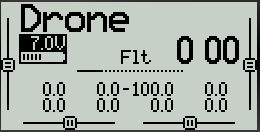
\includegraphics[ width=0.70\linewidth, height=\textheight, keepaspectratio]{./Pictures/taranis-lcd-screenshot.png}
        \caption{\footnotesize Schermata principale del \emph{Taranis QX7S}.}
        \label{fig:taranis-lcd-screenshot}
\end{figure}

La schermata a due colori (chiaro e scuro) rende possibile la lettura di scritte e semplici figure. 

\subsubsection{Display LCD del RadioMaster TX16S}
Il display LCD del \emph{RadioMaster} ha una risoluzione di $480\times272$ pixel e supporta la modalità di colore \texttt{RGB565}. La schermata principale si presenta come in Figura~\ref{fig:radiomaster-lcd-screenshot}. Si può osservare che lo schermo, diversamente dal \emph{Taranis}, supporta una modalità a colori e consente di visualizzare immagini dettagliate di modelli e scritte colorate. La risoluzione è sufficiente per visualizzare figure complesse e scritte di varie dimensioni e colore.

\begin{figure}[ht]
        \centering
        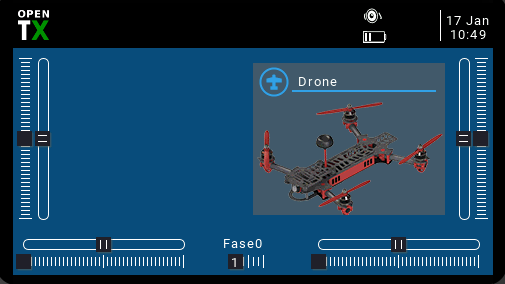
\includegraphics[ width=0.70\linewidth, height=\textheight, keepaspectratio]{./Pictures/radiomaster-lcd-screenshot.png}
        \caption{\footnotesize Schermata principale del \emph{RadioMaster TX16S}.}
        \label{fig:radiomaster-lcd-screenshot}
\end{figure}

\subsubsection{Gestione dello schermo mediante le funzioni \texttt{lcd}}
L'ambiente Lua di OpenTX mette a disposizione dei metodi interni all'oggetto \texttt{lcd} in grado di gestire lo schermo LCD del radiocomando, fornendo un'interfaccia tra di esso ed lo script in Lua. Tali metodi possono essere invocati soltanto dai tipi di script per cui è prevista la possibilità di modificare lo schermo, ovvero dagli \emph{one-time scripts}, dai \emph{telemetry scripts} e dai \emph{widget} per i radiocomandi che li supportano.

\begin{table}
        \begin{center}
                \begin{tabular}{|l|r|}
                        \hline
                        \textbf{FLAG} & \textbf{Descrizione}\\
                        \hline
                        \hline
                        \texttt{0} & Testo normale, nessuna cifra decimale\\
                        \hline
                        \texttt{DBLSIZE} & Testo a dimensione doppia\\
                        \hline
                        \texttt{MIDSIZE} & Testo a dimensione intermedia\\
                        \hline
                        \texttt{SMLSIZE} & Testo a dimensione piccola\\
                        \hline
                        \texttt{INVERS} & Colore di testo e sfondo invertito\\
                        \hline
                        \texttt{BLINK} & Testo lampeggiante\\
                        \hline
                        \texttt{XXLSIZE} & Testo a dimensione molto grande\\
                        \hline
                        \texttt{LEFT} & Testo giustificato a sinistra\\
                        \hline
                        \texttt{RIGHT} & Testo giustificato a destra\\
                        \hline
                        \texttt{PREC1} & Singola cifra decimale per i numeri\\
                        \hline
                        \texttt{PREC2} & Doppia cifra decimale per i numeri\\
                        \hline
                        \texttt{GREY\_DEFAULT} & Lo sfondo del testo è grigio\\
                        \hline
                        \texttt{TIMEHOUR} & Mostra le ore\\
                        \hline
                \end{tabular}
        \end{center}
        \caption{Lista dei possibili flag per i metodi dell'oggetto \texttt{lcd}.}
        \label{tab:elenco-flag-lcd}
\end{table}

I metodi che sono stati adoperati per la gestione dell'interfaccia grafica nella realizzazione degli script sono i seguenti:
\begin{itemize}
        \item \texttt{lcd.clear([color])}: metodo utilizzato negli script di telemetria per resettare la schermata prima di effettuare operazioni di stampa su schermo. Il comando accetta come argomento, opzionalmente, un colore con cui effettuare l'azzeramento della schermata, qualora lo schermo supportasse la modalità a colori. Tale metodo \emph{non è necessario} negli script Widget;
        \item \texttt{lcd.drawText(x, y, text, [flags])}: stampa su schermo la stringa di testo \texttt{text}, alla posizione orizzontale \texttt{x} e verticale \texttt{y}. L'elenco dei \texttt{flag} disponibili è indicato nella tabella~\ref{tab:elenco-flag-lcd};
        \item \texttt{lcd.drawTimer(x, y, value, [flags])}: stampa su schermo un timer con valore in secondi \texttt{value}, alla posizione orizzontale \texttt{x} e verticale \texttt{y}. L'elenco dei \texttt{flag} disponibili è indicato nella tabella~\ref{tab:elenco-flag-lcd};
        \item \texttt{lcd.drawScreenTitle(title, page, pages)}: stampa su schermo il titolo della schermata \texttt{title}, al numero di pagina \texttt{page} e con numero totale di pagine \texttt{pages};
        \item \texttt{lcd.setColor(area, color)}: per gli schermi in grado di supportare i colori, assegna un colore \texttt{color} alla porzione di schermo indicata dalla costante \texttt{area}. In questa tesi, per il valore di \texttt{area} è stata utilizzata la costante \texttt{CUSTOM\_COLOR};
        \item \texttt{lcd.drawFilledRectangle(x, y, w, h, [flags])}: disegna un rettangolo pieno, alla posizione orizzontale \texttt{x} e verticale \texttt{y} e di ampiezza \texttt{w} ed altezza \texttt{h}. L'elenco dei \texttt{flag} disponibili è indicato nella tabella~\ref{tab:elenco-flag-lcd}.
\end{itemize}










\section{OpenTX Companion}

\emph{OpenTX Companion} è un software di supporto per il firmware OpenTX, sviluppato dallo stesso gruppo di sviluppatori che si occupa del firmware. Esso è un programma scritto in C++ e sviluppato per Linux, macOS e Windows che consente la configurazione del radiocomando direttamente da computer, senza incorrere nelle limitazioni imposte dalla dimensione della schermata della radio. OpenTX Companion è infatti adoperato per svolgere vari compiti, come il caricamento del firmware sul radiocomando, eseguire il backup delle impostazioni dei modelli, della scheda SD e del firmware, modificare le configurazioni del radiocomando e condurre delle simulazioni del radiocomando~\cite{opentx-companion-manual}. Quest'ultimo compito è svolto grazie al simulatore \emph{OpenTX Simulator}, incluso nel software Companion.

\subsection{Specifiche e compilazione del sorgente}
Per questa tesi è stato adoperato il sistema operativo Fedora Linux 33~\cite{fedora-website}, con la versione 2.3.11 di OpenTX Companion compilata da codice sorgente.
La compilazione del software è avvenuta dapprima installando le necessarie dipendenze, successivamente clonando il repository di opentx ed infine eseguendo lo script di compilazione \texttt{build-companion-release.sh}. Opzionalmente, è possibile eseguire un'istruzione che modifica in tale script la riga dove è definito il numero totale di unità di calcolo impiegate per la compilazione, modificandolo da $2$ al massimo numero disponibile nella macchina allo scopo di velocizzare il processo di compilazione. Sono stati eseguiti i seguenti comandi:

\begin{lstlisting}
# Installazione delle dipendenze
sudo dnf -y install sed make cmake git gcc gcc-c++ gcc-arm-linux-gnu avr-gcc-c++ avr-gcc xsd bc python python3-pyqt4-sip PyQt4-qsci-api python3-PyQt4-devel python3-pillow python3-pillow-devel avr-libc qt5-qttools qt5-qttools-devel qt5-qtmultimedia qt5-qtmultimedia-devel qt5-linguist qt5-qtsvg qt5-qtsvg-devel dfu-util gcc-plugin-devel fox fox-devel fox-utils SDL SDL-devel SDL2 SDL2-devel SDL_sound sdljava arm-none-eabi-gcc-cs arm-none-eabi-gcc-cs-c++ arm-none-eabi-newlib rpmdevtools rpm-build

# Clone del repository
git clone --recursive -b 2.3 https://github.com/opentx/opentx.git

# Modifica opzionale del numero di jobs
sed -i 's/JOBS=2/JOBS=\$\(nproc\)/g' ./tools/build-companion-release.sh

# Script per la compilazione
./tools/build-companion-release.sh ../ ./build 23
\end{lstlisting}

Al termine dell'esecuzione dell'ultimo comando, OpenTX sarà correttamente compilato all'interno della cartella \texttt{build}. Sarà possibile eseguire il programma con \texttt{./build/companion23}.

Alternativamente, è fornito un eseguibile per Windows, Ubuntu o macOS nella relativa pagina web di download\cite{opentx-download-page}.

\subsection{Utilizzo e funzionalità}

\begin{figure}[ht]
        \centering
        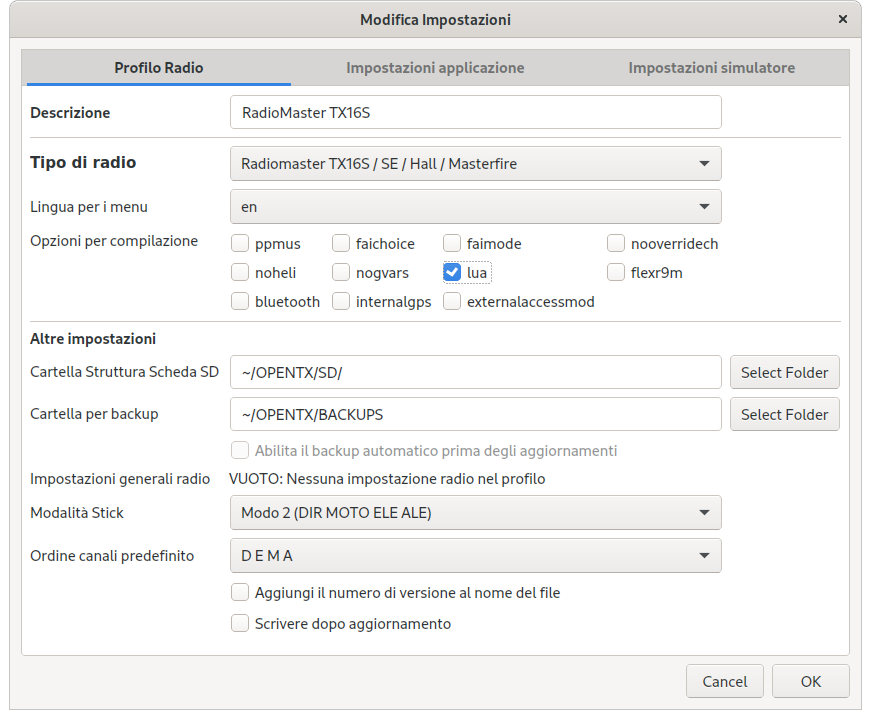
\includegraphics[ width=0.80\linewidth, height=\textheight, keepaspectratio]{./Pictures/opentx-first-config.png}
        \caption{\footnotesize Finestra di prima configurazione di OpenTX Companion.}
        \label{fig:opentx-first-config}
\end{figure}

Al primo avvio di OpenTX Companion è presente una finestra introduttiva, dove viene richiesta una prima configurazione di un profilo di radiocomando. Si seleziona il modello di radiocomando desiderato, nel nostro caso \emph{Taranis QX7S} oppure \emph{RadioMaster TX16S}, e si assegna una breve descrizione al profilo. Successivamente, si include il supporto agli script Lua selezionando la relativa casella e si indica il percorso dove verranno collocati i contenuti della scheda SD, ed opzionalmente, il percorso per i backup. Le restanti impostazioni sono lasciate ai loro valori predefiniti.

La schermata principale di OpenTX Companion si presenta come in Figura~\ref{fig:opentx-main}. Prima di poter simulare un modello, è necessario scaricare il firmware e i contenuti della scheda SD. Per fare ciò, si naviga sull'icona di ``Download'' nella barra degli strumenti per procedere con lo scaricamento. I contenuti della scheda SD andranno poi decompressi con un programma di gestione di file \texttt{.zip} e collocati nella posizione precedentemente indicata.

\begin{figure}[ht]
        \centering
        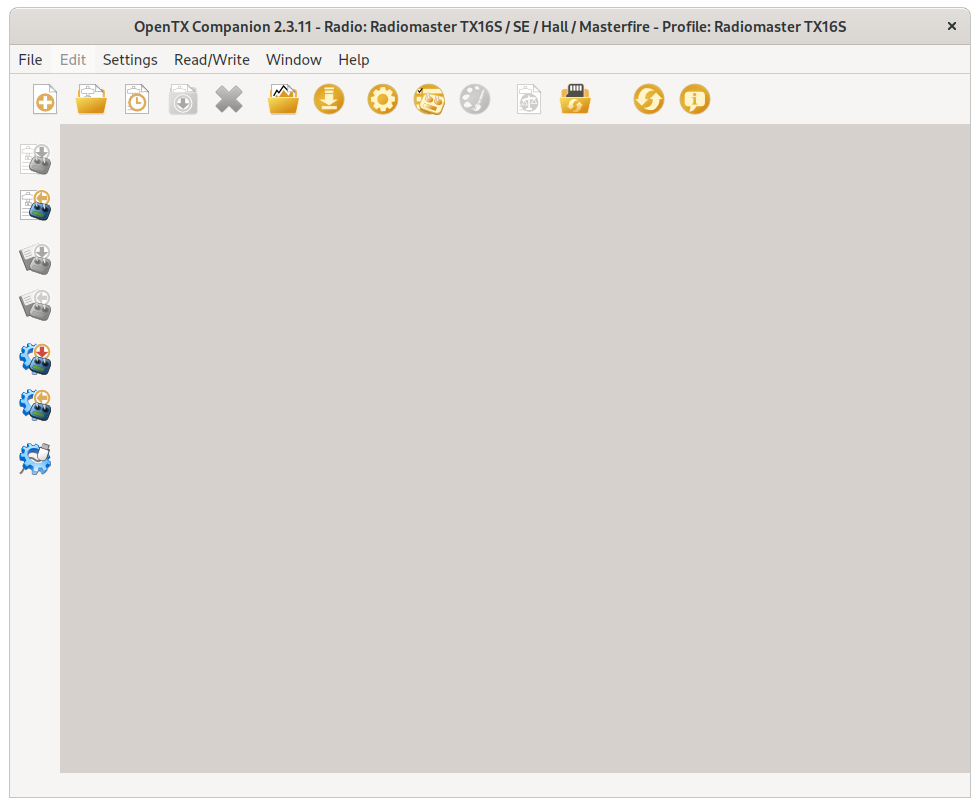
\includegraphics[ width=0.80\linewidth, height=\textheight, keepaspectratio]{./Pictures/opentx-main.png}
        \caption{\footnotesize Finestra principale di OpenTX Companion.}
        \label{fig:opentx-main}
\end{figure}

Prima di simulare il proprio radiocomando è necessario creare un nuovo documento in OpenTX, e collocarvi almeno un modello. Si naviga sull'icona ``New'' nella barra degli strumenti e si aggiunge un nuovo modello con ``Add Model'' all'interno della finestra che è stata aperta. Il wizard di configurazione del modello guiderà l'utente nella selezione delle sue specifiche. È possibile configurare ulteriormente le opzioni della radio in ``Edit Radio Settings'' prima di lanciare la simulazione. In tale menù è possibile applicare varie configurazioni, calibrazioni e funzionalità specifiche come la possibilità di implementare delle \emph{Global Functions}, azioni da eseguire al verificarsi di un evento (ad esempio, una leva è in una determinata posizione o il pilota aziona un determinato bottone).


\begin{figure}[ht]
        \centering
        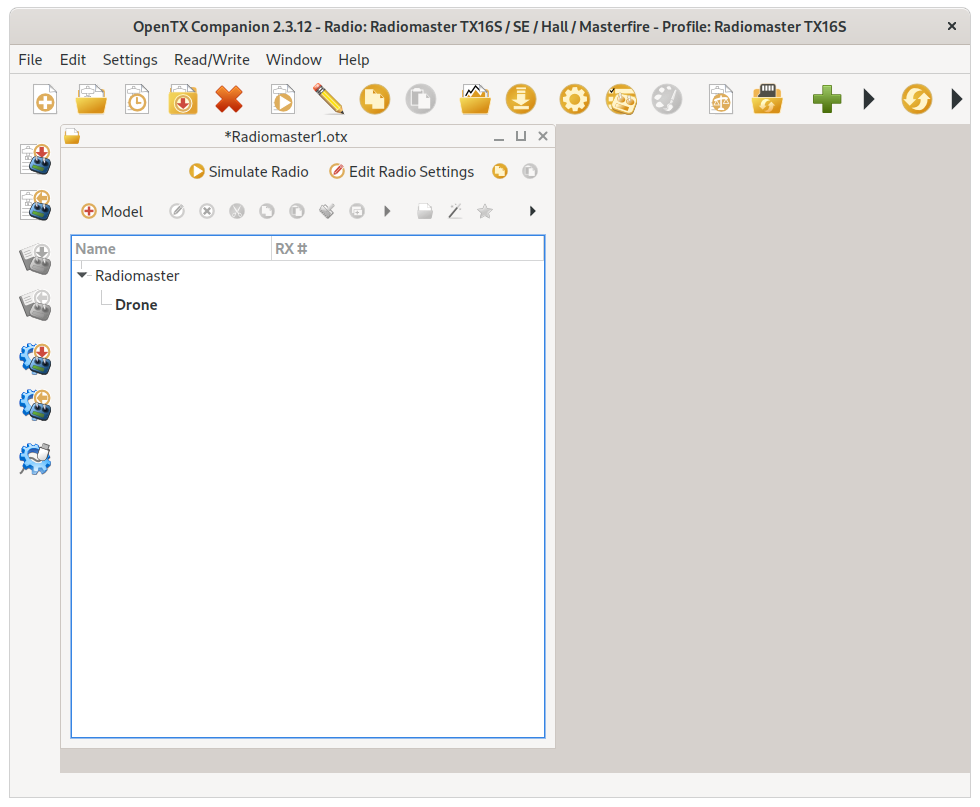
\includegraphics[ width=0.80\linewidth, height=\textheight, keepaspectratio]{./Pictures/opentx-document.png}
        \caption{\footnotesize Creazione di un documento in OpenTX Companion.}
        \label{fig:opentx-document}
\end{figure}

Terminata la configurazione, è possibile eseguire la simulazione con \emph{OpenTX Simulator} navigando su ``Simulate Radio''. Una nuova finestra con il simulatore ci mostrerà una rappresentazione del radiocomando con le necessarie leve, pulsanti ed una riproduzione della schermata. La navigazione all'interno dei menù e delle schermate della radio avviene con i medesimi pulsanti utilizzati per il radiocomando reale. Poiché i vari tipi sono rappresentati il più fedelmente possibile, le modalità di navigazione e le schermate presentate possono differire notevolmente fra i vari modelli di radiocomando.


\begin{figure}[ht]
        \centering
        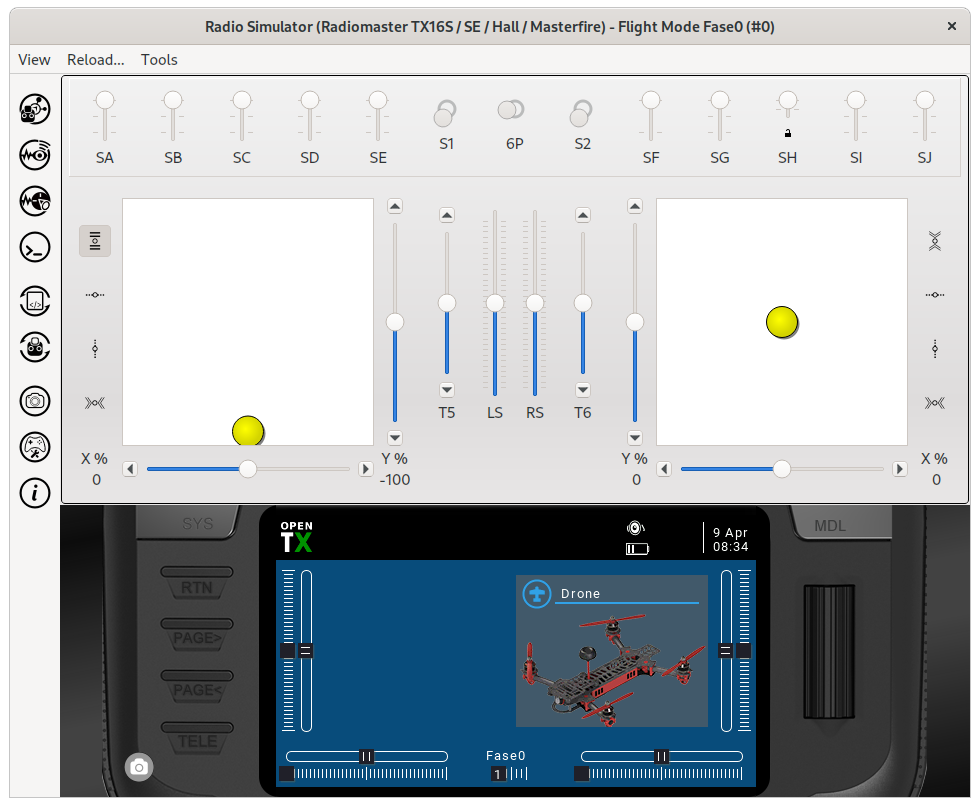
\includegraphics[ width=0.80\linewidth, height=\textheight, keepaspectratio]{./Pictures/opentx-sim-first.png}
        \caption{\footnotesize Simulazione del radiocomando \emph{RadioMaster TX16S} in OpenTX Simulator.}
        \label{fig:opentx-sim-first}
\end{figure}

\begin{figure}[ht]
        \centering
        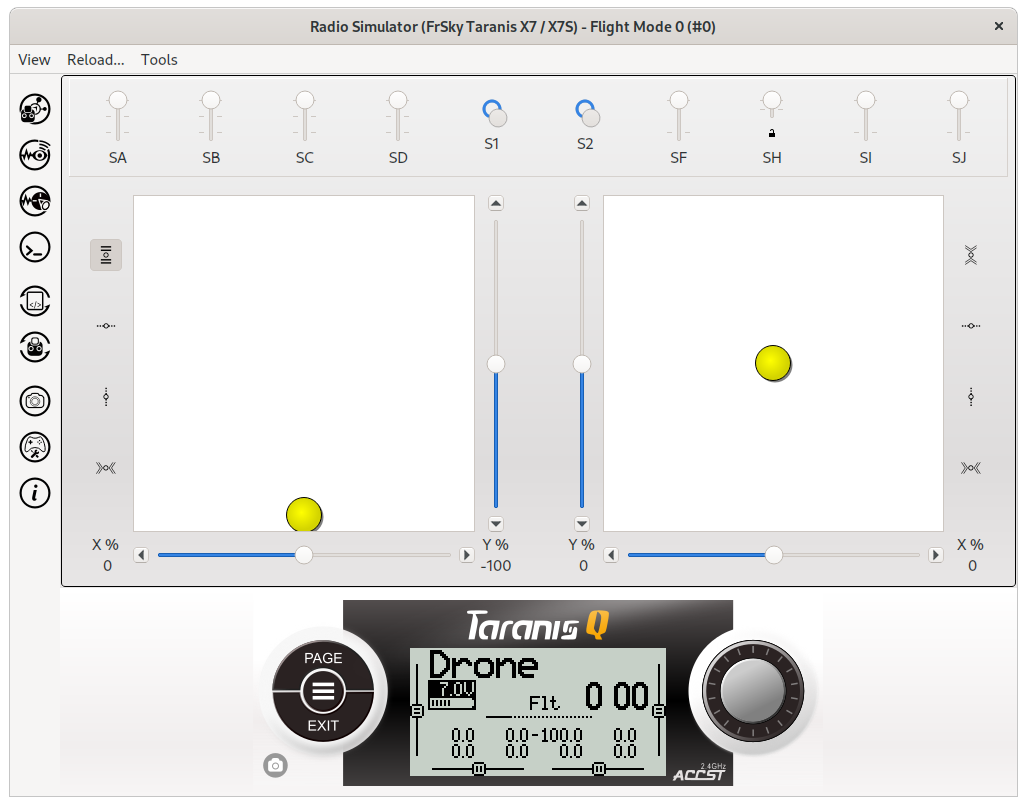
\includegraphics[ width=0.80\linewidth, height=\textheight, keepaspectratio]{./Pictures/opentx-sim-qx7s.png}
        \caption{\footnotesize Simulazione del radiocomando \emph{Taranis FrSky QX7S} in OpenTX Simulator.}
        \label{fig:opentx-sim-qx7s}
\end{figure}

Degna di nota è la schermata di configurazione dei modelli. Per ciascuno di esso infatti, navigando sul nome del modello, tasto destro del mouse, ``Edit Model'', è possibile accedere alla configurazione avanzata del modello. Tramite il proprio computer difatti è possibile impostare:
\begin{itemize}
        \item   i \emph{timer}, sistemi di radio interni ed esterni, il \emph{trainer}, nome ed immagine di modello~\cite{opentx-companion-model-setup};
        \item   le \emph{modalità di volo}~\cite{opentx-companion-flight-modes};
        \item   gli \emph{input}, i \emph{mixer} e gli \emph{output};
        \item   le \emph{curve}~\cite{opentx-companion-curves};
        \item   i \emph{logical switches}, interruttori logici utilizzati per comparare valori e combinare il verificarsi di varie condizioni~\cite{opentx-companion-logical-switches};
        \item   le \emph{special functions}~\cite{opentx-companion-special-functions};
        \item   la \emph{telemetria}.
\end{itemize}

Per il \emph{Taranis FrSky QX7S} è stato necessario configurare due schermate di telemetria, una per ciascuno dei due script Lua trattati in questa tesi. Nel caso del \emph{RadioMaster TX16S}, invece, si è fatto uso della configurazione dei Widget direttamente dall'interfaccia del radiocomando in fase di simulazione.

\chapter{RISULTATI E DISCUSSIONE}
In questa tesi sperimentale sono stati creati due script Lua per ciascuno dei modelli di radiocomando adoperati, il \emph{Taranis FrSky Qx7S} ed il \emph{RadioMaster TX16S}.
\section{Lo script di cronometro vocale}


\subsection{Widget TmrCnt su RadioMaster TX16S}
\subsection{Schermata di telemetria TmrCnt su Taranis QX7S}
\section{Lo script di conto alla rovescia vocale}
\subsection{Widget CntDwn su RadioMaster TX16S}
\subsection{Schermata di telemetria CntDwn su Taranis QX7S}
\chapter{CONCLUSIONI}
\chapter{SVILUPPI FUTURI}



%% Marco Sgobino
%% Tesi di laurea triennale
% file-bibliografia.tex
\titleformat{\chapter}[display]
{\Huge\bfseries}{}{0pt}{}
\clearpage
\addcontentsline{toc}{chapter}{Bibliografia}
\begin{thebibliography}{9}
        \bibitem{opentx-website} OpenTX, \underline{https://www.open-tx.org/}, 2014.
        \bibitem{opentx-radios} OpenTX, \underline{https://www.open-tx.org/radios}, 2014.
        \bibitem{opentx-github} Repository OpenTX su GitHub, \underline{https://github.com/opentx/opentx}, 2021.
        \bibitem{oss-osh-uavs} Burdziakowski, P., Razmjooy, N., Estrela, V., \& Hemanath, J. (2020). \emph{``Open-source software (OSS) and hardware (OSH) in UAVs''}. 49-66
        \bibitem{mission-planner-website} ArduPilot Dev Team, \underline{https://ardupilot.org/planner/}, 2021.
        \bibitem{ardupilot-website} ArduPilot, \underline{https://ardupilot.org/}, 2016.
        \bibitem{opendronemap} OpenDroneMap Authors ODM, \emph{``A command line toolkit to generate maps, point clouds, 3D models and DEMs from drone, balloon or kite images.''} \underline{https://github.com/OpenDroneMap/ODM}, 2020.
        \bibitem{webodm-website} UAV4GEO, \underline{https://webodm.net/}.
        \bibitem{rise-uavs} Cummings, Anthony R.; McKee, Arlo; Kulkarni, Keyur; Markandey, Nakul, \emph{``The Rise of UAVs''}, Photogrammetric Engineering \& Remote Sensing, Volume 83, Number 4, April 2017, pp. 317-325(9)
        \bibitem{italy-uavs} Andrea Cardamone, \emph{``Implementation of a pilot in the loop simulation environment for UAV development and testing''}, \underline{http://hdl.handle.net/10589/135202} 2017.
        \bibitem{opentx-firmware} OpenTXU, \underline{http://open-txu.org/home/undergraduate-courses/introduction/how-rc-works/}, 2014.
        \bibitem{opentx-lua-instructions} OpenTX, \underline{https://www.open-tx.org/lua-instructions.html}, 2014.
        \bibitem{lua-website} Lua Project, \underline{https://www.lua.org/}, 2020.
        \bibitem{opentx-companion-manual} OpenTX, \underline{https://doc.open-tx.org/manual-for-opentx-2-2/companion}.
        \bibitem{fedora-website} Fedora Project, \underline{https://getfedora.org/}, 2021.
        \bibitem{opentx-download-page} OpenTX, \underline{https://www.open-tx.org/downloads}, 2014.
\end{thebibliography}

% https://www.ingentaconnect.com/content/asprs/pers/2017/00000083/00000004/art00016#
% https://mostwiedzy.pl/pl/publication/open-source-software-oss-and-hardware-osh-in-uavs,152706-1
% https://www.politesi.polimi.it/handle/10589/135202?mode=complete


\end{document}
